\chapter*{Ejercicio 1}
\addcontentsline{toc}{chapter}{Ejercicio 1}

\section{Problema 2b de la guía 1}
Utilizando transformada Z sobre toda la red obtenemos:
\begin{figure}[H]
    \centering
    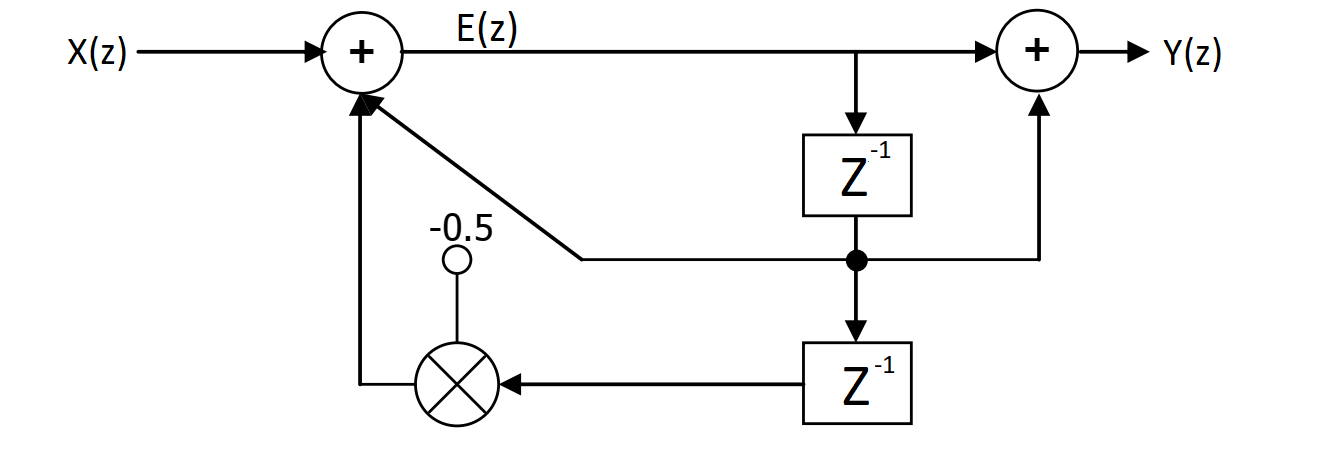
\includegraphics[width=0.5\textwidth]{RedEje1a.png}
    \caption{Red del ejercicio 2b de la guía 1}
\end{figure}
Obtenemos las siguientes formulas:
\begin{equation*}
\left\{
\begin{aligned}
Y(z) & = E(z) + E(z)Z^{-1} \\
E(z) & = X(Z) + E(z)Z^{-1} -0,5 E(Z)Z^{-2}
\end{aligned}
\right.
\end{equation*}
Al re-acomodar las ecuaciones obtenemos:
\begin{equation*}
\left\{
\begin{aligned}
Y(z) & = E(z)\left( 1 + Z^{-1} \right)\\
X(z) & = E(z)\left( 1 -Z^{-1}+0,5Z^{-2} \right)
\end{aligned}
\right.
\end{equation*}
Finalmente obtenemos:
$$\frac{Y(z)}{X(z)}=\frac{1+Z^{-1}}{1 -Z^{-1}+0,5Z^{-2}}$$
$$Y(z)\left( 1 -Z^{-1}+0,5Z^{-2} \right)=X(z)\left( 1 + Z^{-1} \right)$$
Finalmente obteniendo al anti-transformar la siguiente ecuación diferencial:
$$y(nT)-y(nT-T)+0,5y(nT-2T)=X(nT)+X(nT-T)$$

\section{Problema 9 de la guía 1}
Utilizo transformada Z en la red y obtengo:
\begin{figure}[H]
    \centering
    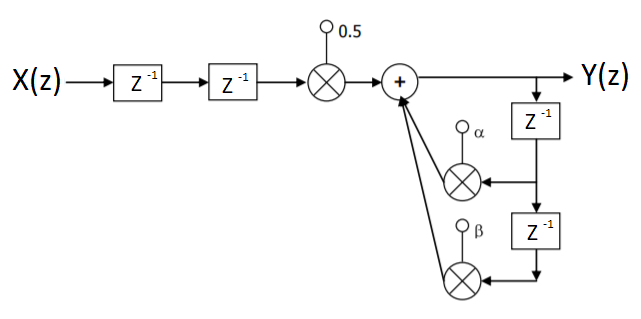
\includegraphics[width=0.5\textwidth]{RedEje9.png}
    \caption{Red del ejercicio 9 de la guía 1}
\end{figure}
Analizando la red obtenemos la siguiente ecuacion:
$$Y(z)= \frac{1}{2} Z^{-2}X(z)+ Y(z) \left( \alpha Z^{-1} + \beta Z^{-2} \right) $$
$$\frac{Y(z)}{X(z)}= \frac{ \frac{1}{2} Z^{-2} } {1- \alpha Z^{-1} - \beta Z^{-2} } $$
$$H(z)=\frac{Y(z)}{X(z)}= \frac{ \frac{1}{2} } {Z^{2}- \alpha Z^{1} - \beta } $$

Vamos a tener 2 polos en:
\begin{equation*}
\left\{
\begin{aligned}
P_1 & = \frac{\alpha + \sqrt{\alpha^2+ 4\beta}}{2}\\
P_2 & = \frac{\alpha - \sqrt{\alpha^2+ 4\beta}}{2}
\end{aligned}
\right.
\end{equation*}
